\subsection{ARIMA}

\begin{frame}{Situation}
	\begin{figure}[]
		%\centering
		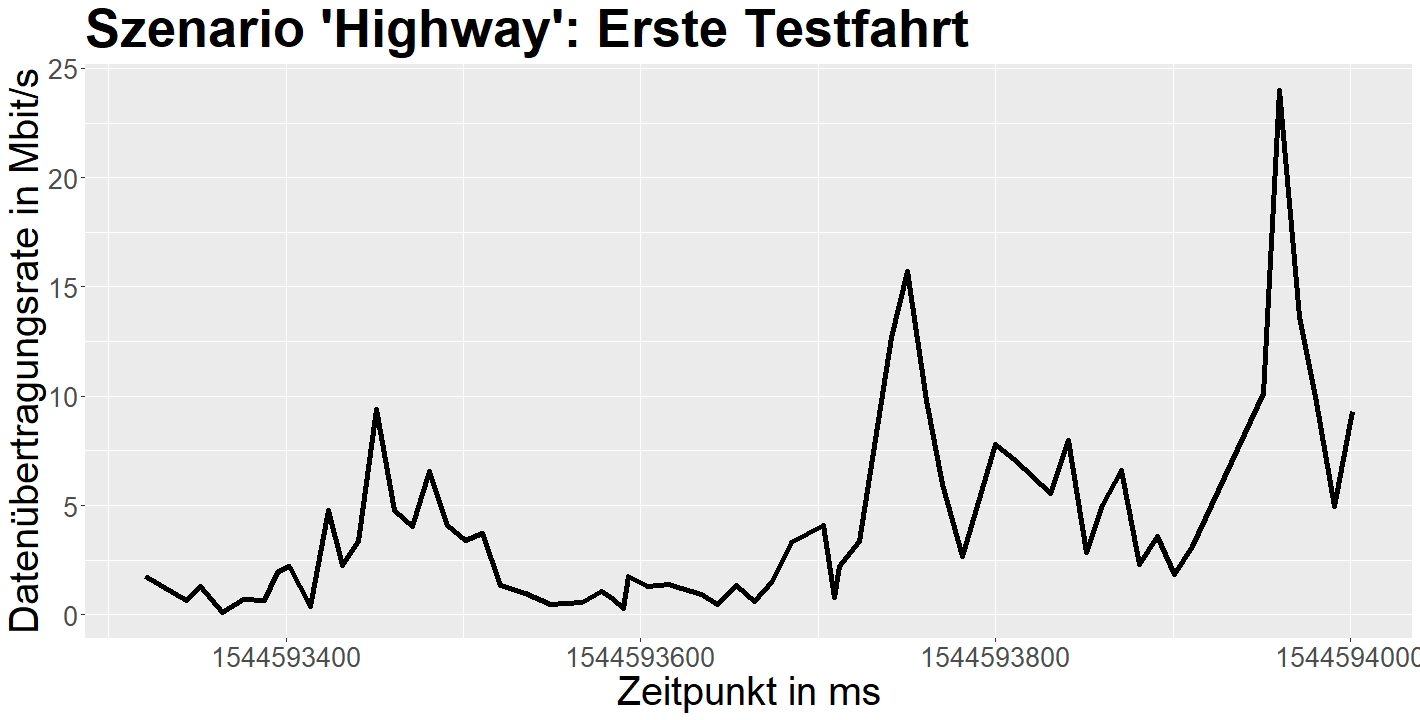
\includegraphics[scale=0.25]{highway_drive_one}
		\caption{Grafik der auf der ersten Testfahrt im Szenario ``Highway'' gemessenen Datenübertragungsrate.}
		\label{highway_drive_one}
	\end{figure}
	
	\begin{itemize}
		\item Zeitreihe $y_1,...,y_n$ (Zielvariable)
		\item k Zeitreihen $x_{i,1},...,x_{i,n}$ für $i=1,...,k$ (Einflussvariablen)
	\end{itemize}
\end{frame}

\begin{frame}{Regression mit ARMA-Fehlern}
	\textbf{Lineares Regressionsmodell} \\
	$$y_{t} = c + \beta_1 x_{1,t} + ... + \beta_k x_{k,t} + \epsilon_t \text{ mit Fehler } \epsilon_t \text{ und Konstante}c$$ \\
	Annahmen an Fehler:
	\begin{itemize}
		\item $\forall t \in \{1,...,n\}: E(\epsilon_t) = 0$
		\item $\forall s, t \in \{1,...,n\} s\neq t: Cov(\epsilon_s, \epsilon_t)=0 $
		\item $Cov((\epsilon_1,...,\epsilon_n)^T)=\sigma^2 \mathds{1}_n$
	\end{itemize}
	\textbf{Annahmen sind in unserer Situation nicht einhaltbar!}
\end{frame}

\begin{frame}{Regression mit ARMA-Fehlern}
	\textbf{ARMA(p, q)}
	Zusammengesetzes Modell aus
	\begin{itemize}
		\item $AR(p)$ (Auto Regressive): $y_{t} = c + \phi_1 y_{t-1} + ... + \phi_p y_{t-p} + e_t \text{ mit Fehler }e_t\text{ und Konstante}c$
		\item $MA(q)$ (Moving Average): $y_{t} = c + e_t + \theta_1 e_{t-1} + ... + \theta_q e_{t-q}\text{ mit White Noise }e_t,e_{t-1},...,e_{t-q}\text{ und Konstante }c$
	\end{itemize}
	Zusammengesetzt:
	$$y_{t} = c + \underbrace{\phi_1 y_{t-1} + ... + \phi_p y_{t-p}}_{AR(p)} + \underbrace{\theta_1 e_{t-1} + ... + \theta_q e_{t-q}}_{MA(q)} + e_t$$
\end{frame}

\begin{frame}{Regression mit ARMA-Fehlern}
	\textbf{Anwendung auf Regressionsfehler} \\
	\underline{Erinnerung}: Fehler $\epsilon_t$ des linearen Modells sind autokorreliert $\Rightarrow$ erfüllen Voraussetzungen nicht\\
	\underline{Lösung}: Wende ARMA-Modell auf Fehler an
	$$\epsilon_{t} = c + \phi_1 \epsilon_{t-1} + ... + \phi_p \epsilon_{t-p} + \theta_1 e_{t-1} + ... + \theta_q e_{t-q} + e_t$$
	\textbf{Modellgleichung Regression mit ARMA-Fehlern}:
	$$y_t = c + \sum_{i=1}^{k}{\beta_i x_{i,t}} + \underbrace{\sum_{j=1}^{p}{\phi_j\epsilon_{t-j}}}_{\text{vergangene Fehler LM}} + \underbrace{\sum_{k=1}^{q}{\theta_k e_{t-k}}}_{\text{vergangene Fehler ARMA}} + e_t$$
	
\end{frame}

\begin{frame}{Regression mit ARMA-Fehlern}
	\textbf{h-Schritt Punktvorhersage}\\
	\begin{itemize}
		\item Ersetze Beobachtungen zu zukünftigen Zeitpunkten mit deren Vorhersagen
		\item Ersetze Fehler an vergangenen Zeitpunkten durch das entsprechende Residuum
		\item Ersetze Fehler an zukünftigen Zeitpunkten durch 0
	\end{itemize}
	\underline{Beispiel}: $h=2, k=1, p=2, q=2$
	\begin{alignat*}{2}
		y_t &= c + \beta_1 x_{t} + \epsilon_t \text{ mit }&&\epsilon_{t} = \phi_1\epsilon_{t-1} + \phi_2\epsilon_{t-2} + \theta_1e_{t-1} + \theta_2e_{t-2} + e_t \\		
		\widehat{y_{t+1}} &= c + \beta_1 x_{t} + \widehat{\epsilon_{t+1}} \text{ mit }&& \widehat{\epsilon_{t+1}} = \phi_1\epsilon_{t} + \phi_2\epsilon_{t-1} + \theta_1e_{t} + \theta_2e_{t-1} + \underbrace{\widehat{e_{t+1}}}_{=0}\\
		\widehat{y_{t+2}} &= c + \beta_1 x_{t} + \widehat{\epsilon_{t+2}}\text{ mit }&&\widehat{\epsilon_{t+2}} = \phi_1\widehat{\epsilon_{t+1}} + \phi_2\epsilon_t + \theta \underbrace{\widehat{e_{t+1}}}_{=0} + \theta e_t + \underbrace{\widehat{e_{t+2}}}_{=0}
	\end{alignat*}
\end{frame}

\begin{frame}{Validierung}
	\textbf{k-fache Kreuzvalidierung}
	\begin{itemize}
		\item beachtet Abhängigkeit der Datenpunkte nicht
		\item zerstört zeitliche Komponente
		\item verwendet eventuell zukünftige Beobachtungen für Prognose der Gegenwart
	\end{itemize}
	$\Rightarrow$ \textbf{Kreuzvalidierung für Zeitreihen}
\end{frame}
	
%\begin{frame}{Validierung}
	%\begin{figure}[h]
	%	\centering
%		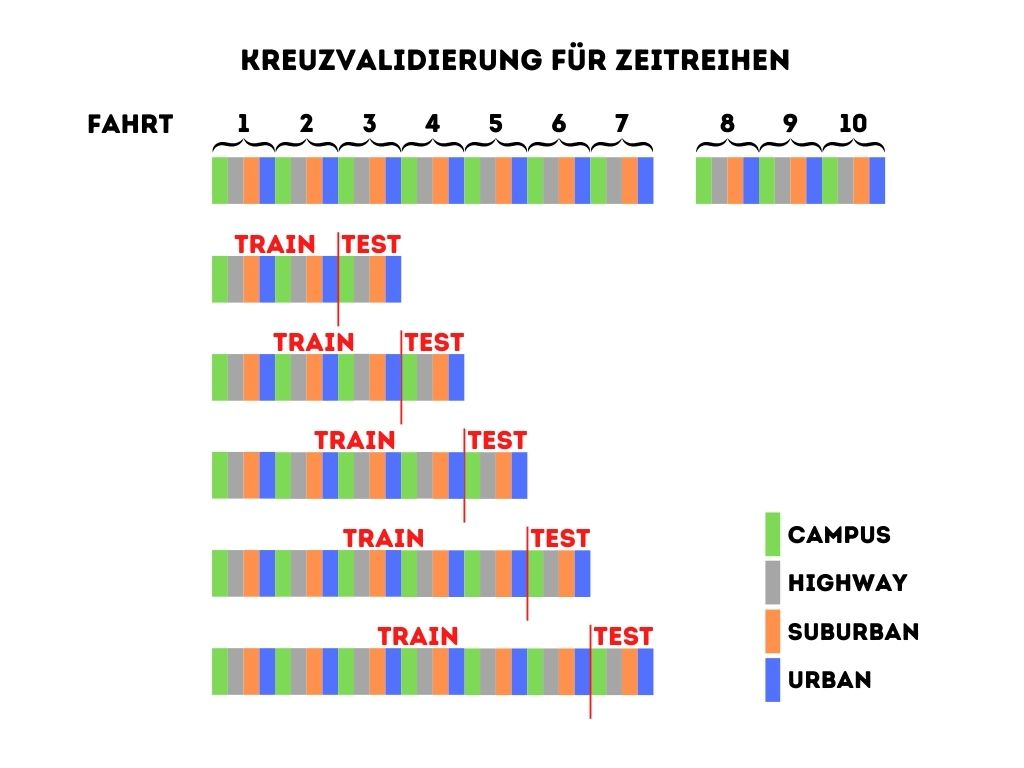
\includegraphics[scale=0.25]{kreuzvalidierung}
		%\caption{Grafik der auf der ersten Testfahrt im Szenario ``Highway'' gemessenen Datenübertragungsrate.}
		%\label{kreuzvalidierung}
	%\end{figure}
%\end{frame}
	


